% useful commands
% \medskip , \smallskip, \noindent, \vspace{0.2in}
% \sc (all caps)
%




\documentclass[11pt]{article}   % For Latex2e
\usepackage{amssymb,amscd,latexsym}   % For Latex2e
\usepackage{amsmath}
\usepackage{amsthm}
\usepackage{epsfig}
\usepackage{enumerate}
\usepackage{listings}
\usepackage{moreverb}
\usepackage{amssymb} % for \smallsetminus

\usepackage{mathtools} % allows you to use \boxed or \Aboxed
\usepackage{mhchem}
%%%%%%%%%%
%\topmargin=-0.5cm
%\marginparwidth=2cm
\textwidth=6.3in
\textheight=22cm
\hoffset=-1.8cm
\voffset=-1.3cm
%%%%%%%%%%%%%%%%%%%
\def\vdotfill{
\vbox to 2em
{\cleaders\hbox{.}\vfill}}
%------------------------

\usepackage{listings}
\usepackage{color}

\definecolor{dkgreen}{rgb}{0,0.6,0}
\definecolor{gray}{rgb}{0.5,0.5,0.5}
\definecolor{mauve}{rgb}{0.58,0,0.82}
\newcommand{\dcomment}[1]{\textcolor{red}{#1}}
\lstset{frame=, %tb
  language=Java,
  aboveskip=1mm,
  belowskip=1mm,
  showstringspaces=false,
  columns=flexible,
  basicstyle={\small\ttfamily},
  numbers=none,
%  numberstyle=\tiny\color{gray},
%  keywordstyle=\color{blue},
  commentstyle=\color{dkgreen},
  escapeinside={\%*}{*)},
  stringstyle=\color{mauve},
  breaklines=true,
  breakatwhitespace=true,
  tabsize=3
}

\newtheorem{Theorem}{Theorem}[section]
\newtheorem{Lemma}[Theorem]{Lemma}
\newtheorem{Corollary}[Theorem]{Corollary}
\newtheorem{Proposition}[Theorem]{Proposition}
\newtheorem{Remark}[Theorem]{Remark}
\newtheorem{Example}[Theorem]{Example}
\newtheorem{Conjecture}[Theorem]{Conjecture}
\newtheorem{Definition}[Theorem]{Definition}
\newtheorem{Question}[Theorem]{Question}
%%%%%%%%%%%%%%%%%%%%%%%%%%
\newcommand{\rar}{\rightarrow}
\newcommand{\lar}{\longrightarrow}
\newcommand{\llar}{-\kern-5pt-\kern-5pt\longrightarrow}
\newcommand{\surjects}{\twoheadrightarrow}
\newcommand{\injects}{\hookrightarrow}
\newcommand{\Fiber}{{\cal F}}

\renewcommand{\phi}{\varphi}
\newcommand{\demo}{{\sc Proof. }}
\renewcommand{\proof}{\demo}
%\newcommand{\demo}{\noindent{\sc Proof. }}
%\newcommand{\square}{\mathchoice\sqr64\sqr64\sqr{4}3\sqr{3}3}
%\newcommand{\qed}{\hspace*{\fill} $\square$}
%\newcommand{\QED}{\hbox{\qed}}





\newcommand{\restr}{{\kern-1pt\restriction\kern-1pt}}




\begin{document}

\begin{center}

\vspace{3in}
{\Huge{\bf\sc Evolution Three}}\\
\vspace{.1in}
{\small\sc ECE 458}


\vspace{0.3in}



{\large\sc Parker Hegstrom} {\large (eph4)} \\
{\large\sc Peter Yom} {\large (pky3)} \\
{\large\sc Wayne You} {\large (wxy)} \\
{\large\sc Brandon Chao} {\large (bc105)} \\


\end{center}


\vspace{0.2in}

\begin{abstract}
In this evolution, we added two new features to our shared calendar web application. Specifically, a user can now create Slot Sign Up events, which allow other users to ``sign up" for an appointment. The second feature is more a service as it allows the user to determine who has event conflicts given certain time frames. In addition to these new features, some major back-end refactoring was done and will be further explained in the following document.
\end{abstract}

\tableofcontents


\pagebreak


\section{Overall Design}

The overarching design principle we wanted to achieve was modularity. In doing so, we believed we would be able to work separately (with occasional meetings to work through minor problems with the API) and refactor without the worry of breaking another members code. Figure \ref{design} below shows a high level diagram of how we decided to design our calendar web application.

\begin{figure}[htb]
\centering
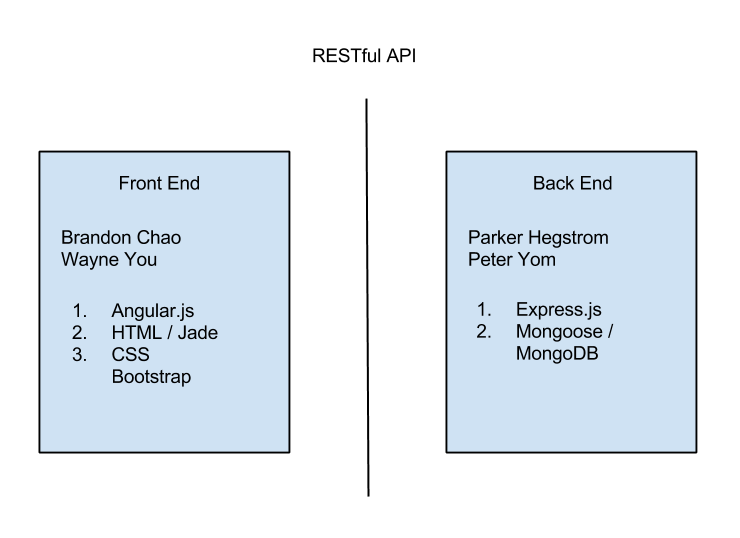
\includegraphics[width=.5\textwidth]{DesignDiagram.png}
\caption{Diagram of our Large Scale Design}
\label{design}
\end{figure}

\noindent Essentially, our back end team provides an exhaustive RESTful API service to our front end. As we received the new requirements for evolution two, the benefits of our modular design came to light as we met to discuss both the refactorings from evolution one that needed to be done and the edits to each modules system design in order to account for the added calendar functionality--event requests and persistent until done events.\\

\noindent At the beginning of evolution three, our group spent four days simply refactoring and making large design change decisions. The back-end did undergo one major change as we now handle repeated events differently. This will be further discussed in the following section.\\

\noindent The following sections further discuss design choices and implications of those design choices for both our front end and back end teams. \\

\section{Back End Design and Analysis}
\subsection{New Features}



\subsection{Benefits of Our Previous Design}


\subsection{Drawbacks of Our Previous Design}



\section{Front End Design and Analysis}



\section{Individual Portion}
\subsection*{Parker}

\begin{enumerate} [a)]
\item  {\bf Designing and Conducting Experiments}
\begin{enumerate} [$\cdot$]
\item 
\end{enumerate}
\item  {\bf Analyzing and Interpreting Data}
\begin{enumerate} [$\cdot$]
\item  
\end{enumerate}
\item {\bf Designing System Components}
\begin{enumerate} [$\cdot$]
\item 
\end{enumerate}
\item {\bf Dealing with Realistic Contraints}
\begin{enumerate} [$\cdot$]
\item 
\end{enumerate}
\item  {\bf Teamwork and Team Member Interaction}
\begin{enumerate} [$\cdot$]
\item 
\end{enumerate}
\end{enumerate}

\subsection*{Peter}

\begin{enumerate} [a)]
\item  {\bf Designing and Conducting Experiments}
\begin{enumerate} [$\cdot$]
\item 
\end{enumerate}
\item  {\bf Analyzing and Interpreting Data}
\begin{enumerate} [$\cdot$]
\item  
\end{enumerate}
\item {\bf Designing System Components}
\begin{enumerate} [$\cdot$]
\item 
\end{enumerate}
\item {\bf Dealing with Realistic Contraints}
\begin{enumerate} [$\cdot$]
\item 
\end{enumerate}
\item  {\bf Teamwork and Team Member Interaction}
\begin{enumerate} [$\cdot$]
\item 
\end{enumerate}
\end{enumerate}

\subsection*{Brandon}

\begin{enumerate} [a)]
\item  {\bf Designing and Conducting Experiments}
\begin{enumerate} [$\cdot$]
\item 
\end{enumerate}
\item  {\bf Analyzing and Interpreting Data}
\begin{enumerate} [$\cdot$]
\item  
\end{enumerate}
\item {\bf Designing System Components}
\begin{enumerate} [$\cdot$]
\item 
\end{enumerate}
\item {\bf Dealing with Realistic Contraints}
\begin{enumerate} [$\cdot$]
\item 
\end{enumerate}
\item  {\bf Teamwork and Team Member Interaction}
\begin{enumerate} [$\cdot$]
\item 
\end{enumerate}
\end{enumerate}

\subsection*{Wayne}

\begin{enumerate} [a)]
\item  {\bf Designing and Conducting Experiments}
\begin{enumerate} [$\cdot$]
\item 
\end{enumerate}
\item  {\bf Analyzing and Interpreting Data}
\begin{enumerate} [$\cdot$]
\item  
\end{enumerate}
\item {\bf Designing System Components}
\begin{enumerate} [$\cdot$]
\item 
\end{enumerate}
\item {\bf Dealing with Realistic Contraints}
\begin{enumerate} [$\cdot$]
\item 
\end{enumerate}
\item  {\bf Teamwork and Team Member Interaction}
\begin{enumerate} [$\cdot$]
\item 
\end{enumerate}
\end{enumerate}

%\keywords{Cremona map \and Newton complementary dual \and monoid \and Cohen--Macaulay}

%\vspace{0.2in}




%\begin{align}
%e^{j\theta} = cos(\theta) + jsin(\theta)
%\end{align}

%\begin{figure}[h]
%\begin{center}
%\epsfig{file=StatPlot.eps, width=5in}
%\caption{\label{boxplot} Box plot of the survey data}
%\end{center}
%\end{figure}


%\begin{figure}[h]
%\begin{center}
%\epsfig{file=histogram.eps, width=4in}
%\caption{\label{histogram} Histogram plot of the survey data}
%\end{center}
%\end{figure}

%\begin{table}[h]
%\begin{center}
%\caption{\label{histotable}Table of frequency values from the Histogram} 
%\begin{tabular}{|c|c|}\hline
%{\bf Type of Engineering} & Frequency \\
%BME & 59 \\
%CEE & 6 \\
%ME & 3 \\
%ECE & 10 \\
%Undecided & 1 \\ \hline
%\end{tabular} \\~\\
%\end{center}
%\end{table}

%\begin{figure}[htb]
%\centering
%\includegraphics[width=1.3\textwidth]{Screenshot.png}
%\caption{Screen shot from StatKey}
%\label{samples}
%\end{figure}


%\appendix
%\section{Codes}
%\subsection{MakeGraph.m}
%\listinginput[1]{1}{MakeGraph.txt}


% GIVES TWO TABLES BY EACHOTHER
%\begin{table}[h!]
%\begin{minipage}[b]{0.45\linewidth}\centering
%\caption{\label{ecoli3}Using {\tt ecoli\_edit\_120481.txt}} 
%\begin{tabular}{|c|c|c|}
%\hline
%1 & 1 & 1 \\
%\hline
%\end{tabular}
%\end{minipage}
%\hspace{0.5cm}
%\begin{minipage}[b]{0.45\linewidth}
%\centering
%\caption{\label{ecoli4}Using {\tt ecoli\_edit\_3947161.txt}} 
%\begin{tabular}{|c|c|c|}
%\hline
%1 & 1 & 1 \\
%\hline
%\end{tabular}
%\end{minipage}
%\end{table}



\end{document}
% end of file template.tex

